\begin{document}
% ----------------------------------------
% Deckblatt
% ----------------------------------------
\thispagestyle{empty}
% ----------------------------------------
% LUH Logo                      IMKT Logo
% ----------------------------------------
\begin{tikzpicture}
    \node[anchor=south west, inner sep=0] (imkt) at (0, 0) {
        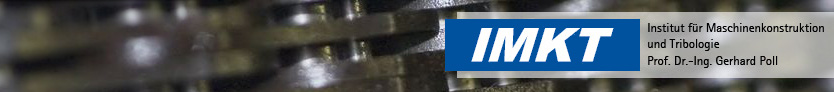
\includegraphics[width=\textwidth]{./images/imkt_logo_small.jpg}
    };

        \begin{scope}[x={(imkt.south east)}, y={(imkt.north west)}]
            %\draw[help lines, xstep=0.1, ystep=0.1] (0, 0) grid (1, 1);
            %\foreach \x in {0, 1, ..., 9} {
            %    \node [anchor=north] at (\x/10,0) {0.\x};
            %}
            %\foreach \y in {0, 1, ..., 9} {
            %    \node [anchor=east] at (0, \y/10,0) {0.\y};
            %}

            \node[anchor=south west, inner sep=0] (luh) at (0.05, 0.15) {
                
\includegraphics[width=4.7cm]{./images/luh_logo.png}
            };
        \end{scope}
\end{tikzpicture}

% ----------------------------------------
% Titel der Arbeit
% ----------------------------------------
\vspace{1cm}

\begin{center}
    \textbf{{\Large Entwicklung eines modularen Messsystems zur optischen und kapazitiven Schmierfilmdickenmessung in einem EHD-Kontakt}}
\end{center}

% ----------------------------------------
% Bild für diese Arbeit
% ----------------------------------------

% ----------------------------------------
% Masterarbeit und VW Logo
% ----------------------------------------
\vspace{12cm}

\begin{center}
    {\textbf{\Large Masterarbeit}}\\[1cm]

    {\large Durchgeführt bei der}

    {\large Volkswagen AG, Wolfsburg}

    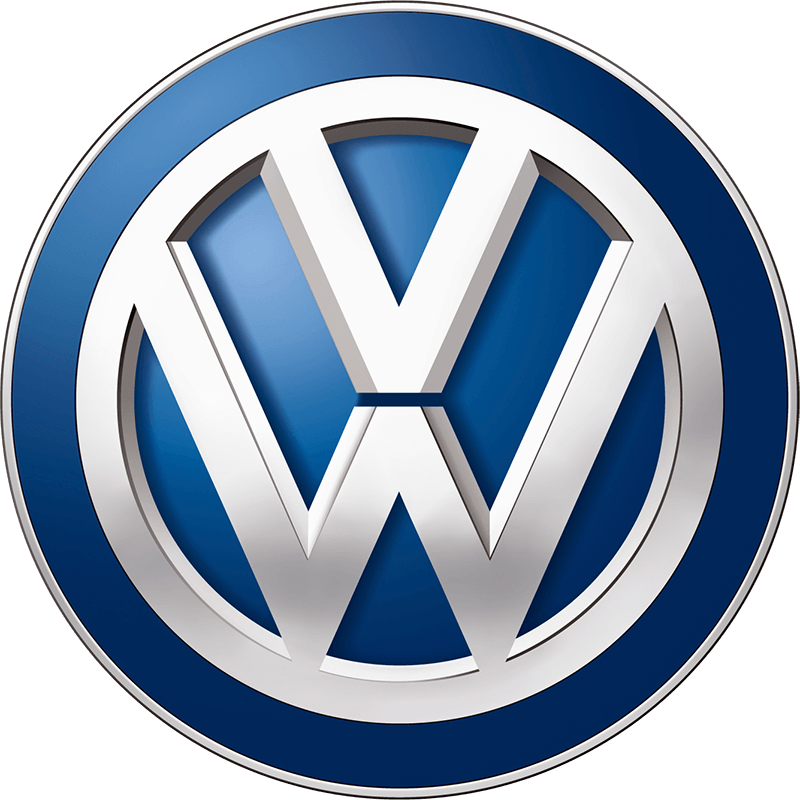
\includegraphics[width=2cm]{./images/vw_logo.png}
\end{center}

% ----------------------------------------
% Verfasser                     Betreuer
% ----------------------------------------
\vfill

\begin{minipage}[t]{0.5\textwidth}
    \begin{flushleft}
        Verfasser:

        cand. mach. Ngoc Minh \textsc{Dao}
    \end{flushleft}
\end{minipage}
%
\begin{minipage}[t]{0.5\textwidth}
    \begin{flushright}
        Betreuer:

        Dipl.-Ing. Norbert \textsc{Bader}
    \end{flushright}
\end{minipage}

% ----------------------------------------
% Seperate line
% ----------------------------------------
\rule{\textwidth}{1pt}

% ----------------------------------------
% Bericht Nr                    Ort, Datum
% ----------------------------------------
\begin{minipage}[t]{0.5\textwidth}
    \begin{flushleft}
        \textbf{Bericht Nr. 1412}
    \end{flushleft}
\end{minipage}
%
\begin{minipage}[t]{0.5\textwidth}
    \begin{flushright}
        \textbf{Hannover, \today}
    \end{flushright}
\end{minipage}



% ----------------------------------------
% Table of contents
% ----------------------------------------
\tableofcontents

% ----------------------------------------
% Einleitung
% ----------------------------------------
\chapter{Einleitung}
\label{chap:einleitung}



% ----------------------------------------
% Stand der Technik
% ----------------------------------------
% ----------------------------------------
% Chapter: Stand der Technik
% ----------------------------------------
\chapter{Stand der Technik}
\label{chap:stand_der_technik}

Ein geschmierter Reibungskontakt kann auf vier Elemente des tribologischen Systems nach Czichos \cite{czihos} reduziert werden:
\begin{itemize}
    \item Grundkörper
    \item Gegenkörper
    \item Zischenstoff
    \item Umgebungsmedium
\end{itemize}

% ----------------------------------------
% Fig: Das tribologische System
% ----------------------------------------
\begin{figure}[htb]
    \centering
    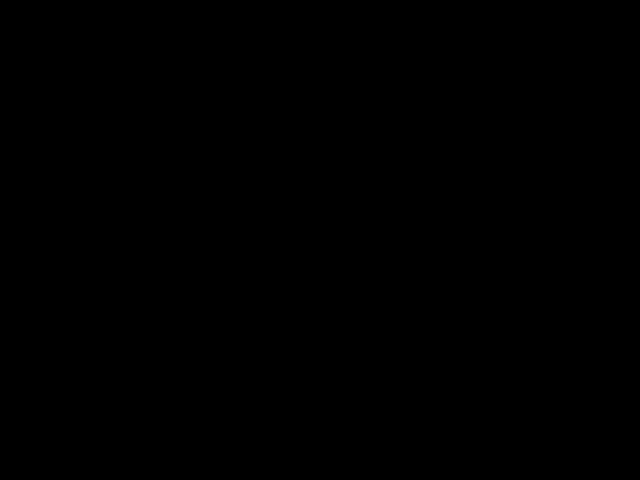
\includegraphics[width=5cm]{./images/blank_img.jpg}
    \caption{Das tribologische System}
    \label{fig:das_tribologische_system}
\end{figure}

Um ein besseres Verständnis der EHD-Schmierung zu haben, wird in diesem Abschnitt die Kennwerte des Zwischenstoffes (Schmiermittel) und der beiden Kontaktelementen (Grund- und Gegenkörper) ausführlich besprochen.

\section{Eigenschaften des Schmiermittels}
\label{sec:eigenschaften_des_schmiermittels}
\begin{itemize}
    \item Viskosität
    \item Kinematische Viskosität
    \item Temperatureffekt
    \item Einfluss von Druck auf Viskosität
    \item Dichte
    \item Brechungsindex
    \item Wärmeleitfähigkeit
    \item Nichtnewtonsches Verhalten
    \item Verfestigung der Schmierung bei hohem Druck
\end{itemize}

\section{Betrachtung des EHD-Kontaktes}
\label{sec:betrachtung_des_ehd_kontaktes}
\begin{itemize}
    \item Nichtkonformer Kontakt
    \item Hertzsche Gesetz
        \begin{itemize}
            \item Kugel-Kugel
            \item Kugel-Platte
        \end{itemize}
    \item Kontakt von beschichteten Körpern
\end{itemize}

\section{Elastohydrodynamische Schmiertheorie}
\label{elastohydrodynamische_schmiertheorie}
Erklärung, wie EHD funktioniert

\section{Schmierfilmdicke nach Hamrock und Dowson}
\label{sec:schmierfilmdicke_nach_hamrock_und_dowson}
Erklärung, wie mann die Schmierfilmdicke berechnen kann



% ----------------------------------------
% Literaturforschung der experimentellen Technik in der EHD Schmierung
% ----------------------------------------
\chapter{Literaturforschung der experimentellen Technik in EHD Schmierung}
\label{chap:literaturforschung_der_experimentellen_technik_in_ehd_schmierung}
% ----------------------------------------
% Optische Methode
% ----------------------------------------
\section{Optische Messung der EHD Schmierfilmdicke}
\label{sec:optische_messung_der_ehd_schmierfilmdicke}

\subsection{Licht Interferometrie}
\label{ssec:licht_interferometrie}

\subsection{Messung der EHD Filmdicke}
\label{ssec:messung_der_ehd_filmdicke}

\subsection{Variante von der klassichen optischen Interferometrie Methode}
\label{ssec:variante_interferometrie}

% ----------------------------------------
% Elektrische Methode
% ----------------------------------------
\section{Elektrische Messung der EHD Schmierfilmdicke}
\label{sec:elektrische_messung_der_ehd_schmierfilmdicke}

\subsection{Kapazitive Methoden}
\label{ssec:kapazitive_methoden}

\subsection{Resistive Methoden}
\label{ssec:resistive_methoden}

% ----------------------------------------
% Alternative Methoden
% ----------------------------------------
\section{Alternative EHD Schmierfilmdicke Messmethoden}
\label{sec:alternative_messmethoden}

\subsection{Ultraschall}
\label{ssec:ultraschall}

\subsection{Laserinduzierte Fluoreszenz}
\label{ssec:laserinduzierte_fluoreszenz}


% ----------------------------------------
% Durchgeführte experimentellen Methoden
% ----------------------------------------
\chapter{Durchgeführte experimentellen Methoden}
\label{chap:durchgefuehrte_experimentellen_methoden}

\section{PCS Instrument Prüfstand}
\label{sec:pcs_pruefstand}

\subsection{Mechanischer Aufbau}
\label{ssec:mechanischer_aufbau}

\subsection{Messsystem zur Schmierfilmdickemessung}
\label{ssec:messsystem_zur_schmierfilmdickemessung}

\section{Versuchte Öle}
\label{sec:versuchte_oele}

\section{Versuchdurchführung}
\label{sec:versuchdurchfuehrung}


% ----------------------------------------
% Versuchergebnisse
% ----------------------------------------
\chapter{Versuchergebnisse}
\label{chap:versuchergebnisse}


% ----------------------------------------
% Diskussion
% ----------------------------------------
\chapter{Diskussion}
\label{chap:diskussion}


% ----------------------------------------
% Zusammenfassung und Ausblick
% ----------------------------------------
\chapter{Zusammenfassung und Ausblick}
\label{zusammenfassung_und_ausblick}

Was soll in die Zusammenfassung sein.

Was ist der Ausblick von dieser Arbeit


% ----------------------------------------
% Literaturverzeichnis
% ----------------------------------------
% Leteraturliste soll im Inhaltsverzeichnis auftauchen
\newpage
\addcontentsline{toc}{chapter}{Literatur}

% Literaturliste
%\bibliography{./literatures/literaturen}

% ----------------------------------------
% Anhang
% ----------------------------------------
\addcontentsline{toc}{chapter}{Anhang}
Anhang:

Bilde, Formelherleitung, Zeichnung etc...



\end{document}
